\section{Appendix: Controllers}
\label{sec:controllers}
\smallskip
\noindent\textbf{Sampled-time Abstraction of Control System.}\
Let $\Sigma = (X, x_\init, U, W, f)$ be a control system and $\tau>0$ be the sampling time.
%(The ``$\cdot$''-s in place of the output space and the output function represent their insignificance in the respective sampled-time abstraction; similar convention will be used elsewhere in the paper.)
A \emph{sampled-time abstraction} of $\Sigma$ is the state-transition system $(X,x_\init,U,f_\tau)$, such that $x'$ is in $f_\tau(x,u)$ if and only if there is a trajectory $\xi\in \Sol_\Sigma(x,u,\tau)$ with $\xi(\tau)=x'$.

The \emph{product sampled-time abstraction} of a set of control systems $\set{\Sigma^i} $ is the product transition system of the set of sampled-time abstractions $\set{\Sigma^i_\tau} $.

\smallskip
\noindent\textbf{Open-loop Controller.}\
Let $\Sigma_\tau=(X,x_\init,U,f_\tau)$ be the sampled-time abstraction of the control system $\Sigma=(X,x_\init,U,W,f)$.
An \emph{open-loop controller of} $\Sigma_\tau$ is a function $C\colon [0;T]\to U$ for some given time horizon $T>0$.
The \emph{open-loop} is obtained when we connect $C$ with $\Sigma_\tau$ serially, and is formalized using the transition system $C \triangleright \Sigma_\tau = (X\times [0;K],x_\init,U,f_\tau^C)$ such that $(x',k+1)$ is in $f_\tau^C((x,k),u)$ if and only if $x'$ is in $f_\tau(x,u)$ and $C(k)=u$.
The \emph{open-loop behavior} $\Beh^\ol(x_\init)$ of $\Sigma_\tau$ under $C$ is the set of all trajectories of the transition system $C \triangleright \Sigma_\tau$.

\smallskip
\noindent\textbf{Feedback Controller.}\
Let $\Sigma_\tau=(X,x_\init,U,f_\tau)$ be the sampled-time abstraction of the control system $\Sigma=(X,x_\init,U,W,f)$.
A \emph{feedback controller of} $\Sigma_\tau$ is a function $C\colon X\times[0;T]\to U$ for a given time horizon $T$.
The \emph{closed-loop} is obtained when we connect $C$ with $\Sigma_\tau$ in feedback, and is formalized using the transition system $C\parallel\Sigma_\tau = (X,x_\init,U,f_\tau^C)$ such that $x'$ is in $f_\tau^C(x,u)$ if and only if $x'$ is in $f_\tau(x,u)$ and $C(x)=u$.
The feedback controller $C$ when connected to the sampled-time control system $\Sigma_\tau$ can be interpreted as a zero-order-hold controller for the control system $\Sigma$.
The \emph{closed-loop behavior} $\Beh^\cl(x_\init)$ of $\Sigma_\tau$ under $C$ is the set of all trajectories of the transition system $C\parallel\Sigma_\tau$.

\smallskip
\noindent\textbf{Local and Global Controller.}\
Let $\set{\Sigma^i} $ be a set of control systems, $\tau >0$ be a given sampling time, $\set{\Sigma^i} $ be the respective sampled-time abstractions, $\Sigma^\times$ be the product control system of $\set{\Sigma^i} $, and $\Sigma^\times_\tau$ be the product sampled time abstraction of $\set{\Sigma^i} $.
A \emph{global} open-loop (feedback) controller of $\set{\Sigma^i} $ is an open-loop (a feedback) controller of $\Sigma_\tau^\times$.
On the other hand, a set of \emph{local} open-loop (feedback) controllers of $\set{\Sigma^i_\tau} $ is a set $\set{C^i} $ where, for every $i\in [1;N]$, $C^i$ is an open-loop (a feedback) controller of $\Sigma^i_\tau$.
\newpage
\subsection{Temporary Figures}

 \begin{figure}[h]
	\centering
	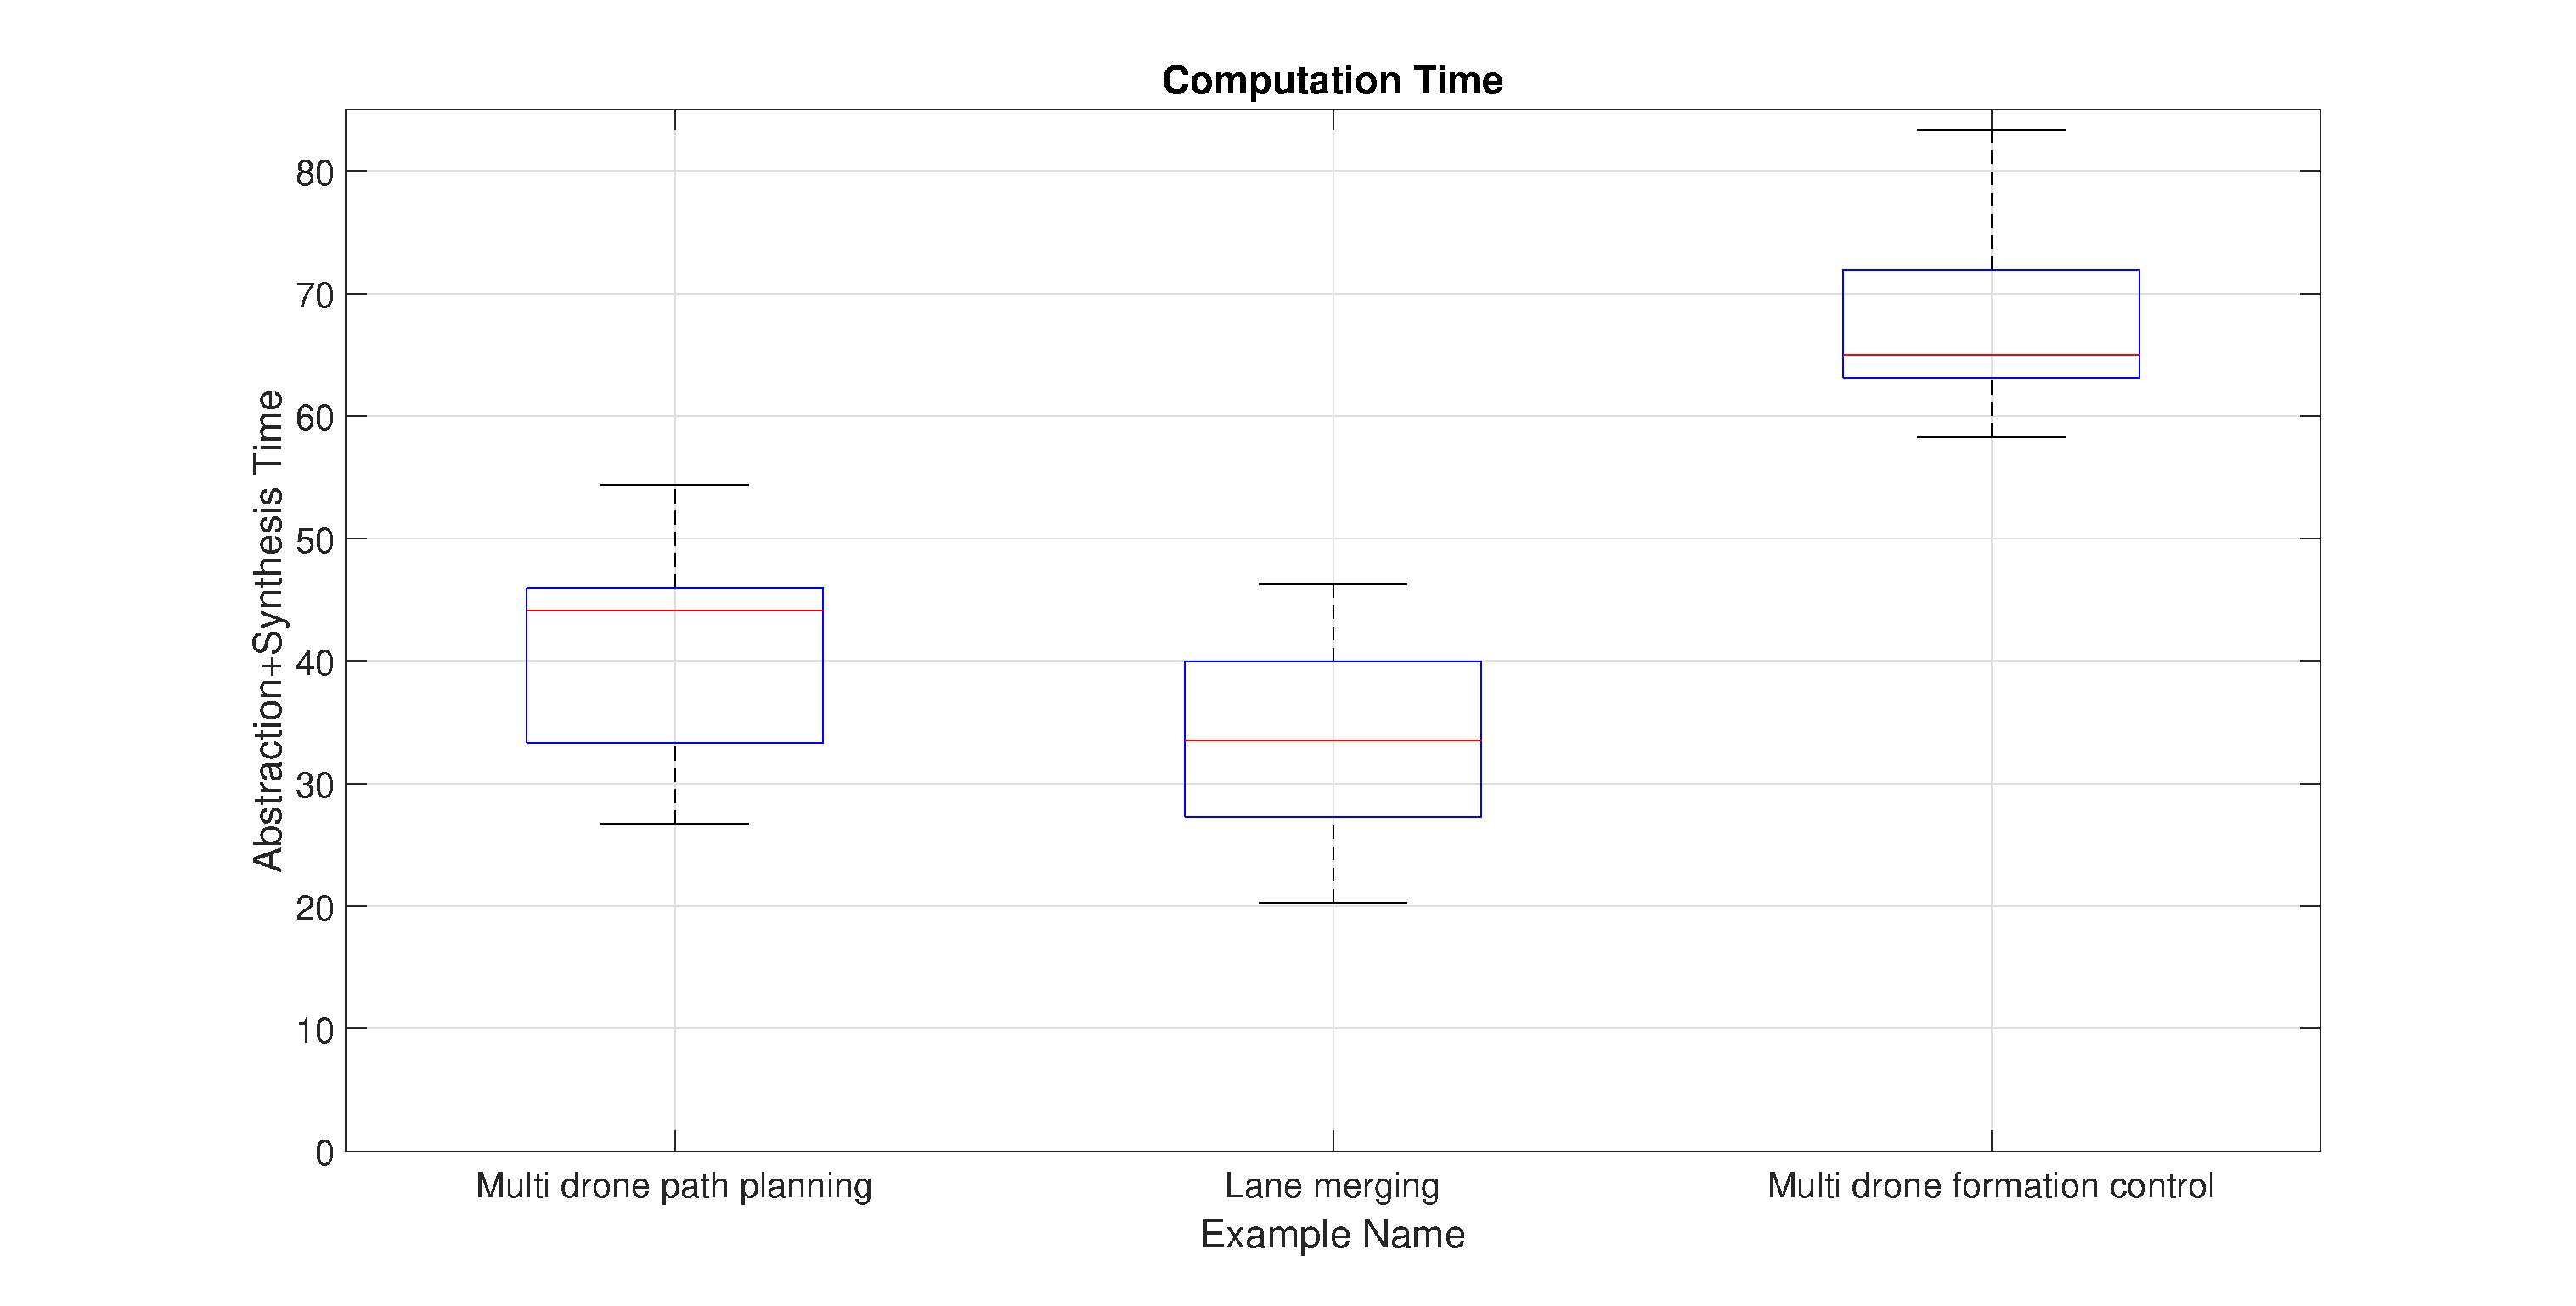
\includegraphics[width=0.45\textwidth]{figures/box1.eps}
	\caption{Box plot for Local ABCD (Abstraction+ synthesis time)}
	\label{fig:Temp1}
\end{figure}
 \begin{figure}[h]
	\centering
	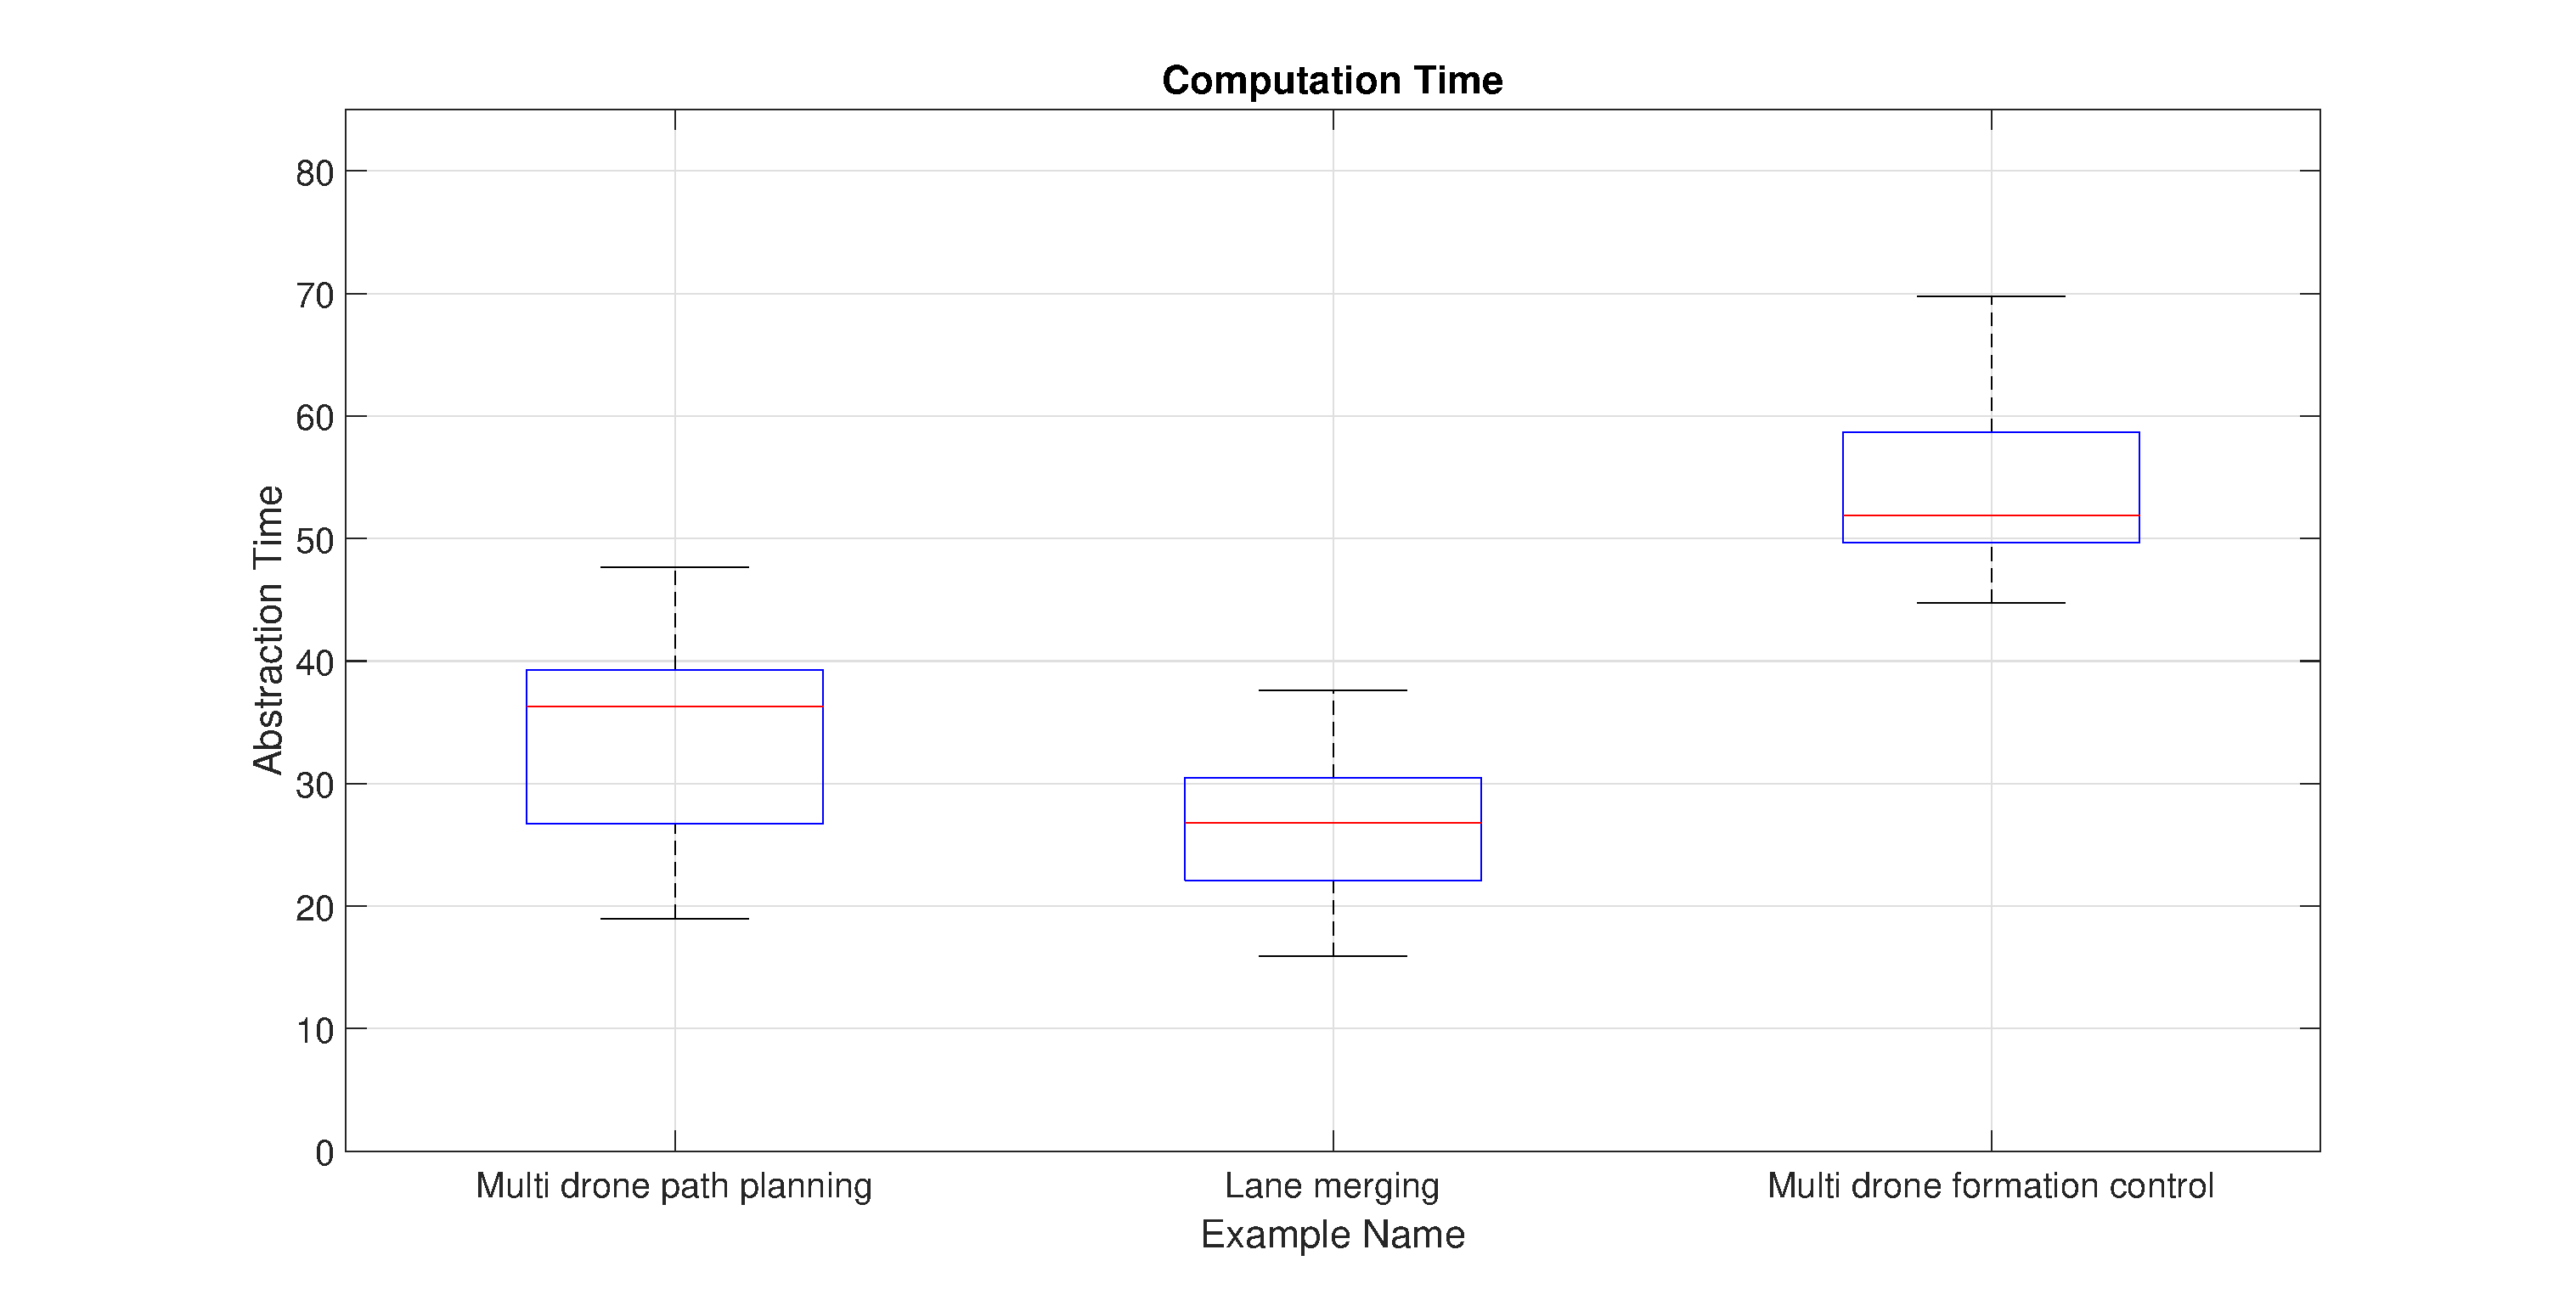
\includegraphics[width=0.45\textwidth]{figures/box2.eps}
	\caption{Box plot for Local ABCD (Abstraction time)}
	\label{fig:Temp2}
\end{figure}
 \begin{figure}[h]
	\centering
	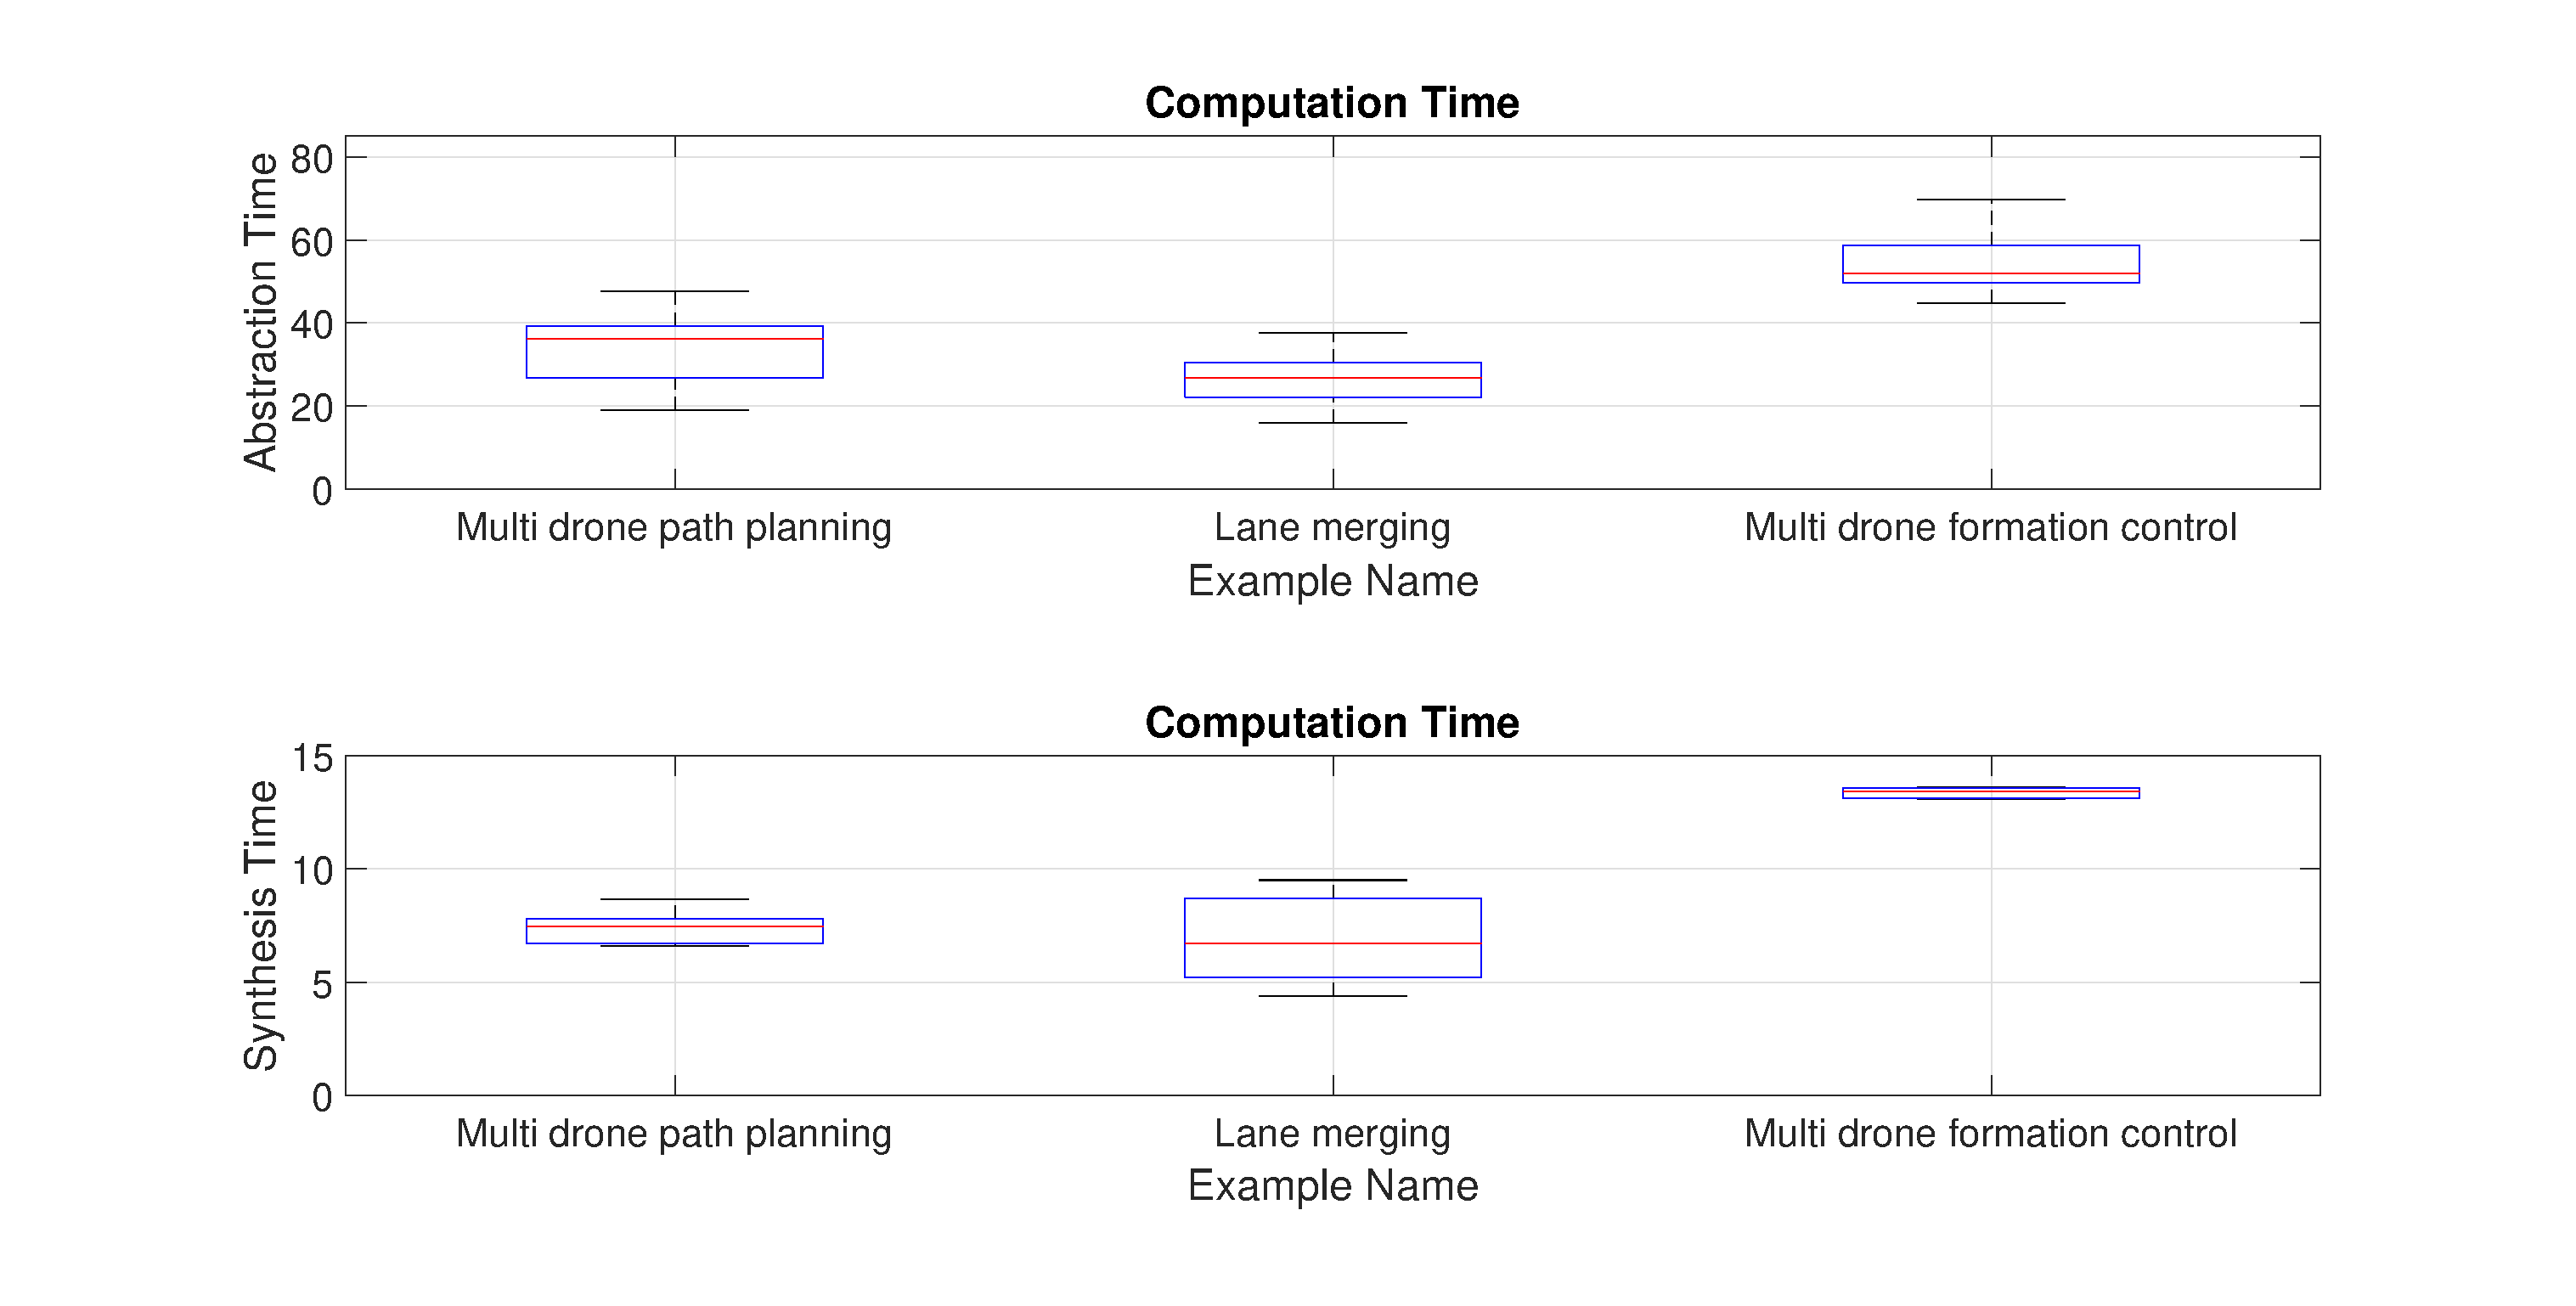
\includegraphics[width=0.45\textwidth]{figures/box3.eps}
	\caption{Box plot for Local ABCD (Abstraction and synthesis time)}
	\label{fig:Temp3}
\end{figure}
 \begin{figure}[h]
	\centering
	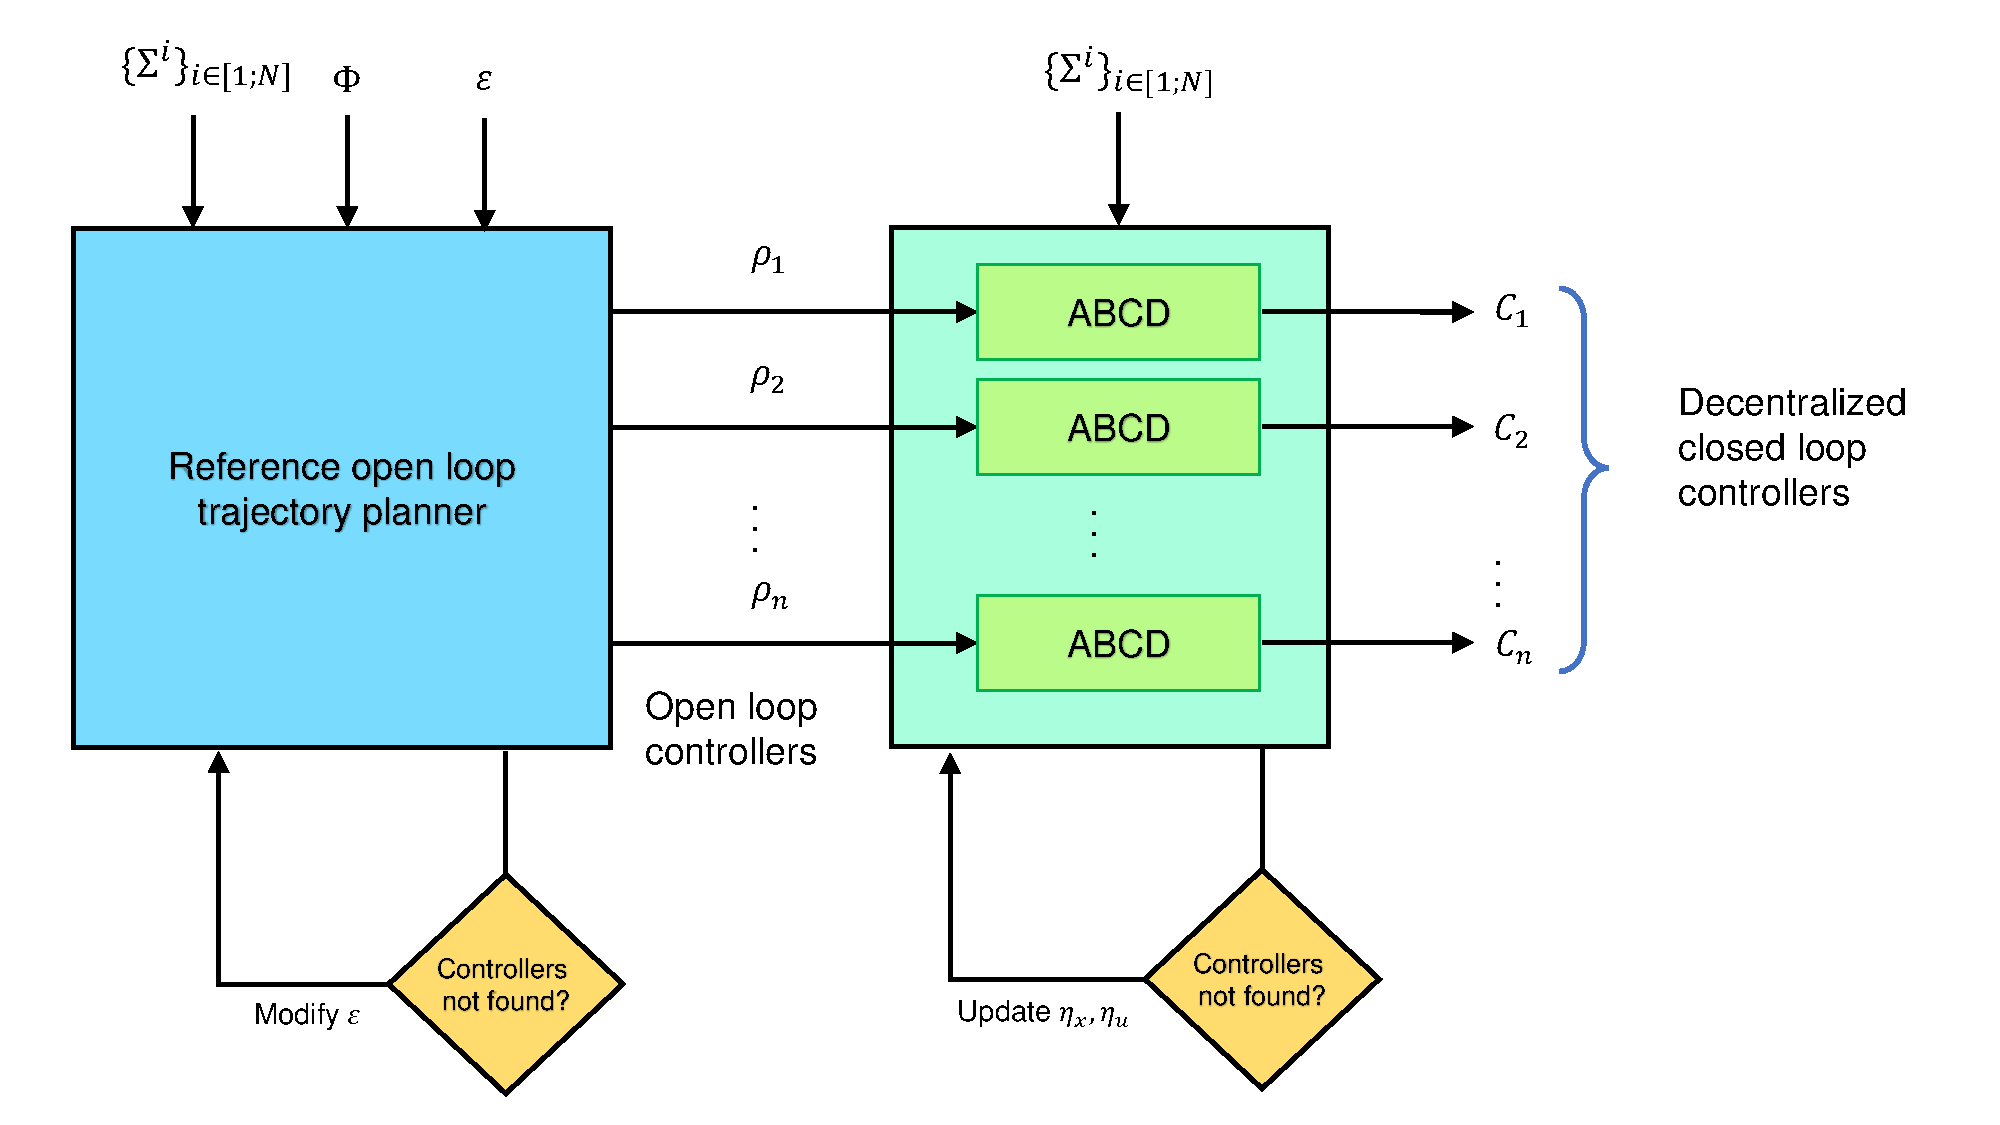
\includegraphics[width=0.45\textwidth]{figures/Algorithm_outline.pdf}
	\caption{Algorithm Outline}
	\label{fig:Temp4}
\end{figure}

%\smallskip
%\noindent\textbf{Decentralized Control.}\
%Given $\set{\Sigma_\tau^i} $ and a set of open-loop (feedback) controllers $\set{C^i} $, we define the \emph{decentralized open-loop} (\emph{decentralized closed-loop})---denoted by $\set{C^i} \triangleright \set{\Sigma_\tau^i} $ ($\set{C^i} \parallel \set{\Sigma_\tau^i} $)---as the product transition system of $\set{C^i\triangleright \Sigma^i_\tau} $ ($\set{C^i\parallel \Sigma^i_\tau} $).
